\documentclass[10pt]{article}
% Public (de-anonymized) build: compile public.tex instead of main.tex.
\newif\ifpublic
\ifdefined\publicbuild
  \publictrue
  \PassOptionsToPackage{preprint}{tmlr}
\else
  \publicfalse
\fi
\usepackage{tmlr}
% If accepted, instead use the following for camera-ready:
% \usepackage[accepted]{tmlr}

\newcommand{\codeurl}{https://github.com/sky-is-green/bonsai2-ternary-forensics}
\ifpublic
  \newcommand{\coderef}{\href{\codeurl}{\texttt{github.com/sky-is-green/bonsai2-ternary-forensics}}}
\else
  \newcommand{\coderef}{the anonymized supplementary material}
\fi

\usepackage{xcolor}
\usepackage[hidelinks]{hyperref}
\ifpublic
  \hypersetup{
    pdfborder={0 0 0},
    colorlinks=true,
    linkcolor=blue!50!black,
    citecolor=green!45!black,
    urlcolor=blue!65!black
  }
\fi
\usepackage{url}
\usepackage{graphicx}
\usepackage{booktabs}
\usepackage{amsmath,amssymb}
\usepackage{microtype}

\newcommand{\R}{\mathbb{R}}
\newcommand{\E}{\mathbb{E}}
\newcommand{\bpw}{\mathrm{bpw}}
\newcommand{\PPL}{\mathrm{PPL}}
\newcommand{\trit}{\mathrm{trit}}
\newcommand{\code}[1]{\texttt{#1}}

% Unnumbered first-page footnote (used for the venue-required LLM disclosure).
\newcommand{\blfootnote}[1]{%
  \begingroup
  \renewcommand{\thefootnote}{}%
  \footnote{#1}%
  \addtocounter{footnote}{-1}%
  \endgroup
}

\title{Forensics on Ternary Bonsai 2 27B: Format Recovery, Trained-Weight Residual, and a Calibration Artifact}

% Authors are hidden in the submission version (no [accepted]/[preprint] option).
\author{\name Ricky Palmer \email ricky.palmer@example.com \\
      \addr Independent Researcher}

\newcommand{\fix}{\marginpar{FIX}}
\newcommand{\new}{\marginpar{NEW}}

\begin{document}

\maketitle

\begin{abstract}
Ternary language models promise roughly two bits per weight, but a released
checkpoint is an opaque artifact: it is not obvious what is verifiable from the
file itself. We perform an independent forensic study of Ternary Bonsai 2 27B,
a $\sim$2\,bpw ternary model built from Qwen3.8-27B. We make four
contributions. First, we recover the storage format and the blockwise
Walsh--Hadamard rotation basis from the released GGUF, reproducing the released
trits from the public base model with plain absmean round-to-nearest at
0.920 mean / 0.885 minimum agreement per tensor (chance 0.33); the recovery is
later confirmed against metadata the authors published separately. Second, we
show the residual is the model: a byte-controlled replacement of all 402 ternary
payloads with rotate-and-round weights of the public base, keeping metadata and
layout byte-identical, collapses held-out perplexity from $18.5851$ to
$23{,}606$ ($1{,}270\times$) in the same binary, corpus and settings. Third, we
falsify the quantizer hypothesis with real activation Hessians: every
error-compensated assignment (GPTQ variants, act-order, rotation-aware
Hessians, group scale search) moves codes \emph{away} from the released ones,
and the released codes fit our Hessians $\sim$7\% worse than plain
round-to-nearest. The residual is trained weight movement. Fourth, we show that
a widely cited public post-training-quantization baseline ($2.1\times$) is a
calibration-passage artifact: the same configurations collapse by
$1{,}178\times$ to $\sim$$35{,}000\times$ on held-out windows. We close the
quantizer reverse-engineering track, report a holdout leak that retracts our own
earlier 1.7B retention figure, and record every falsified route so it can be
re-assessed. No model weights are redistributed.
\end{abstract}

\section{Introduction}
\label{sec:intro}

Weight quantization is now the default way to make large language models
deployable, and the field has settled into two regimes.\blfootnote{Generative
AI tools were used in the preparation of this manuscript. All technical
claims, numbers, and citations were verified by the author against the
recorded reports and public sources, and the author takes full responsibility
for the content.} Post-training
quantization (PTQ) rounds a trained model using calibration statistics, with
error-compensating variants such as GPTQ~\citep{gptq} and rotation-based
preprocessing such as QuIP~\citep{quip}, QuIP\#~\citep{quipsharp},
QuaRot~\citep{quarot} and SpinQuant~\citep{spinquant}. Quantization-aware
training (QAT) instead learns the weights with the quantizer in the loop,
usually with a straight-through estimator~\citep{ste}, sometimes with
distillation~\citep{kd}. Ternary weights---$\{-s, 0, +s\}$, roughly two bits
per weight---sit at the aggressive end of this spectrum, from early ternary
weight networks~\citep{twn} to ternary-native training at scale
\citep{bitnet158}.

A released ternary checkpoint, however, is an opaque object. It reports a bit
width and a benchmark table, but the file itself does not say how the weights
were produced, how much of the quality lives in the released codes rather than
in the quantizer, or whether the recipe is reproducible from the public base
model. This matters: the claims that make a low-bit release interesting are
exactly the claims a user cannot check.

We report an independent forensic study of one such release: Ternary
Bonsai 2 27B, a $\sim$2\,bpw ternary model built from Qwen3.8-27B that ships as
a GGUF and runs on a public inference fork~\citep{prismbonsai2,prismfork,
qwen38}. We do not run the training recipe. We treat the released artifact as
the specimen and the public base model as the control, and we ask four
questions:

\begin{itemize}
  \item \textbf{Q1 (format).} What exactly is the storage format, and can the
  released codes be reproduced from the public base model without access to the
  training code?
  \item \textbf{Q2 (quality).} How much of the model's quality lives in the
  released weights, as opposed to the container or the quantizer?
  \item \textbf{Q3 (mechanism).} Is the residual between a public-base round-to-
  nearest solution and the released codes an error-compensation trick, or
  trained weight movement?
  \item \textbf{Q4 (evaluation).} Does a widely cited public PTQ baseline
  reproduce its published quality when calibration and evaluation are
  separated?
\end{itemize}

\paragraph{Contributions.}
\begin{enumerate}
  \item \textbf{Format and basis recovery} (\S\ref{sec:format}). From the
  released file alone, we recover the blockwise Walsh--Hadamard rotation basis,
  the axis and sign conventions, and the tensor layouts, and reproduce the
  released trits from the public base with plain absmean round-to-nearest at
  $0.920$ mean / $0.885$ minimum per-tensor agreement (chance $0.33$). The
  recovery is later confirmed exactly against metadata the model authors
  published independently: block size, transform, axis, explicit signs, and
  the inverse-rotated embedding all match.
  \item \textbf{The residual is the model} (\S\ref{sec:residual}). A
  byte-controlled, in-place replacement of all 402 ternary payloads with
  rotate-and-round weights of the public base---metadata, layouts, and
  exemptions kept byte-identical---collapses held-out perplexity from
  $18.5851$ to $23{,}606$ ($1{,}270\times$) in the same binary, corpus, and
  settings, even though the replaced codes still agree with the released ones
  on 90--95\% of weights.
  \item \textbf{The residual is trained weight movement} (\S\ref{sec:mechanism}).
  With real activation Hessians captured on a four-layer prefix of the 27B, we
  show that every error-compensated assignment we tried---GPTQ damping sweeps,
  act-order, rotation-aware Hessians, group scale search, stochastic
  calibration---moves codes \emph{away} from the released ones, and that the
  released codes fit our Hessians about 7\% \emph{worse} than plain
  round-to-nearest. The released codes are not an error-compensation of the
  public base; the weights themselves moved.
  \item \textbf{A public PTQ baseline is a calibration artifact}
  (\S\ref{sec:ptq}). We reproduce the published $2.106\times$ figure exactly on
  its fixed calibration passage, and show the same configurations collapse by
  $1{,}178\times$ to $\sim$$35{,}000\times$ on held-out windows with real
  calibration data.
\end{enumerate}

We also settle a mechanistic hypothesis: the large-$q$ mirror-descent /
regularized mirror-descent recipe~\citep{rmd,rmd2,proximalmf} is not the
mechanism behind the released weights (\S\ref{sec:recipe}). Direct tests inside
the ternary loop make it worse at every checkpoint, and the shape argument
explains why: a mirror map forms a single magnitude shell, while ternary needs
mass at both $0$ and $s$. Separately, we retract our own earlier 1.7B retention
figure after finding a holdout leak in our evaluation harness; the corrected,
clean value is reported with its range.

\paragraph{Scope and honesty.}
This is a forensic study of one artifact, not a benchmark suite and not a
replication of the recipe. Section~\ref{sec:limitations} lists the evidence
boundary and every threat to validity we know of, including the fact that some
numbers come from a 1.7B canary rather than the 27B, one corpus, and single
runs. Every falsified route is recorded in the failure register in
Appendix~\ref{app:failures} so that later work can re-assess it. No model
weights are redistributed; all analysis uses publicly released files and the
public base model.

\section{Background and related work}
\label{sec:background}

\paragraph{Ternary and low-bit weight quantization.}
Ternary weight networks~\citep{twn} and the 1.58-bit line
\citep{bitnet158} show that weights in $\{-s, 0, +s\}$ can support useful
language models when training accounts for the quantizer. In practice ternary
storage costs about two bits per weight once group scales and packing are
counted; ``1.58 bits'' is an entropy figure, not a storage width. Group-wise
scales are the standard mechanism that lets a single global ternary alphabet
adapt to per-group weight statistics.

\paragraph{PTQ, error compensation, and rotations.}
PTQ methods round a frozen model using calibration data; GPTQ~\citep{gptq}
chooses codes by minimizing a layer-wise quadratic proxy with a Hessian and
propagates the resulting error to later columns, and QuIP-style methods
\citep{quip,quipsharp} precondition the problem with random or Hadamard
rotations so that weights and Hessians are incoherent before rounding.
Rotations have since become a standard component of low-bit inference stacks
\citep{quarot,spinquant}. A practical pitfall of all of these methods is
calibration: their error metrics and round decisions depend on the passages
used for calibration, and it is not always verified that reported quality
survives when the calibration set and the evaluation set are disjoint. Section
\ref{sec:ptq} studies exactly that failure mode on a public baseline.

\paragraph{QAT and distillation.}
QAT keeps the quantizer in the forward pass and estimates gradients through it,
typically with a straight-through estimator~\citep{ste}; distillation from a
full-precision teacher~\citep{kd} is commonly combined with it. A training
recipe built this way is not recoverable from the released weights by
inspection; the best one can do forensically is test the mechanisms such a
recipe would leave behind.

\paragraph{The Bonsai 2 release and its ecosystem.}
Bonsai 2 27B is a ternary release derived from Qwen3.8-27B, a hybrid-attention
model with gated linear-attention layers interleaved with full attention
\citep{qwen38,qwen3}. The release ships as GGUF and runs on a public
ROCm/CUDA inference fork with a ternary runtime and speculative
decoding~\citep{prismfork,llamacpp,gguf}. The authors separately publish the
format ground truth in an MLX-oriented repository: a Hadamard manifest
(block size, transform, axis, and explicit sign vectors) and the runtime codec
for the packed format~\citep{prismbonsai2mlx}. The surrounding community has
already closed several questions: format and interop are essentially settled,
multiple third-party draft heads and repacks load with parity, and at least one
post-hoc refinement improves the released model by a few percent
perplexity~\citep{gsqrco,mtp,jang}. What the community has not done, at the
time of writing, is retrain ternary weights, and a same-ruler comparison
between trained ternary and PTQ at matched size is still open. This study
contributes on the verification side of that gap.

\section{The released artifact and the forensic toolkit}
\label{sec:artifact}

\paragraph{The specimen.}
Bonsai 2 27B is released as a GGUF of $7.2$\,GB
(sha256 \code{3907dc16\ldots}) derived from the public base model
Qwen3.8-27B at a pinned revision (sha \code{1d4bf0f2\ldots})
\citep{prismbonsai2,qwen38}. The base is a hybrid-attention transformer:
$64$ layers, of which $16$ use full attention (layers $3,7,\dots,63$) and the
rest use gated linear attention. In the released file, $402$ tensors are stored
in the ternary format, comprising $26{,}869{,}760{,}000$ ternary parameters;
the rest of the model---norms, the recurrent state path of the linear-attention
blocks, convolutions, and a handful of small projections---is kept in BF16 or
F32, about $0.0976\%$ of parameters by count. The embedding is ternary as well
and is the only tensor whose rotation is inverted rather than applied; we
return to this in \S\ref{sec:format}.

\paragraph{The packed format.}
The ternary format is the GGUF type-142 layout the release calls
\texttt{PQ2\_0}: a group of $128$ weights is stored in $34$ bytes, with an FP16
group scale in bytes $0$--$1$ and $32$ bytes of packed trits, $16$ trits per
little-endian 32-bit word. Decoding is exact and cheap, which is what makes the
rest of this study possible: we can decode every released payload to a
$\{-1,0,+1\}$ code and a per-group scale without running any model code.

\paragraph{The rotation hypothesis.}
Rotation-based quantization is standard in this literature
\citep{quip,quipsharp,quarot,spinquant}, so the first question is whether the
released codes are a rotate-and-round quantization of the public base. The
family we test is:

\begin{equation}
  R \;=\; \frac{1}{\sqrt{n}}\, H_n \, \mathrm{diag}(S),
  \label{eq:rotation}
\end{equation}

\noindent with $n=1024$, $H_n$ the normalized Sylvester Walsh--Hadamard
transform, $S$ an explicit $\pm 1$ sign vector stored per tensor in the file
metadata, and the transform applied along the input axis of each linear layer.
We treat the axis, the order of the sign and Hadamard steps, the block size, and
whether norms are folded into the rotation as hypotheses to falsify, and score
each hypothesis by the per-tensor trit agreement

\begin{equation}
  \eta(W, W^{\star}) \;=\; \frac{1}{|W|}\sum_i \mathbf{1}\!\left[\trit(W_i) = W_i^{\star}\right],
  \label{eq:agreement}
\end{equation}

\noindent where $W^{\star}$ are the decoded released trits and $\trit(\cdot)$
is the round-to-nearest ternary map under the stored group scale. The chance
level is $1/3$: a mismatched convention scores an agreement at chance, while a
correct one scores far above it, so the metric is a sharp discriminator.

\paragraph{The controlled payload swap.}
Agreement measures how many codes match; it does not measure whether the matched
codes recover quality. To make the quality question causal we patch the released
file in place: decode each of the $402$ payloads, replace the trits with a
rotate-and-round quantization of the corresponding public-base tensor, re-pack
byte-exactly, and keep every other byte of the file---metadata, tokenizer,
tensor table, layouts, exemptions, offsets---unchanged. The result is a
same-binary, same-format, same-runtime comparison in which only the ternary
payloads vary.

\paragraph{Hessians from a prefix.}
Testing error-compensated quantizers requires real activation statistics, but
the 27B does not fit in local memory ($55.6$\,GB of weights against $40$\,GB of
VRAM plus roughly $20$\,GB of usable RAM). We therefore load only the embedding
and layers $0$--$3$ ($55$ tensors) and capture float32 Hessians on real corpus
windows, which is sufficient for the layer-wise GPTQ family; this ``prefix
trick'' is validated by the fact that the tests of
\S\ref{sec:mechanism} are layer-local, and by the direction of their results
across all tested tensors.

\paragraph{Evaluation protocol.}
Quality numbers throughout the paper use the release's inference fork and its
perplexity binary on a fixed corpus (Tiny Shakespeare~\citep{tinyshakespeare},
$\sim$1.1\,MB, $8\times512$ context, one process at a time), plus a five-prompt
smoke test for sanity. The protocol is deliberately small and identical across arms, so that
the comparisons are controlled; its limits are stated in
\S\ref{sec:limitations}. Runtime timings come from the same fork and are
reported only descriptively.

\paragraph{Falsification-first bookkeeping.}
Every route we tested is recorded in a failure register with its claim, method,
outcome, and the cost to re-assess it (Appendix~\ref{app:failures}). Several
entries are negative results we consider as informative as the positive ones,
including one retraction of our own earlier number
(\S\ref{sec:recipe}). The register is append-only: corrections are appended,
not rewritten.

\section{Recovering the format and the rotation basis}
\label{sec:format}

\paragraph{The basis is recoverable.}
Plain absmean round-to-nearest of the rotated public base, with the convention
of Equation~\ref{eq:rotation}, reproduces the released trits at
$0.920$ mean / $0.885$ minimum agreement over $26$ tensors sampled from layers
$0$, $3$, $62$, and $63$ (Table~\ref{tab:gate1}). Chance is $0.33$; a
$1.7$B-era public release of the same family measured $0.612$ under the same
metric, so the $0.92$ is not an artifact of the metric but a property of the
correct basis. Getting there required four conventions to be right
simultaneously, visible as a cliff in the table: the transform is applied on
the input axis, the sign multiplication happens before the Hadamard transform,
the block size is $1024$ with per-block explicit signs, and norms are not
folded into the rotation. Any other combination lands at chance.

\begin{table}[t]
\caption{Per-tensor trit agreement of rotate-and-round hypotheses against the
released codes (mean over tensors; chance $1/3$). Only the input-axis,
sign-then-Hadamard, explicit-signs convention recovers the codes.}
\label{tab:gate1}
\begin{center}
\begin{tabular}{lc}
\toprule
hypothesis & agreement $\eta$ \\
\midrule
no rotation (plain absmean RTN) & $0.333$ \\
output-axis rotation & $\sim 0.33$ \\
FWHT-then-sign order & $\sim 0.33$ \\
sign-then-FWHT, input axis, block $1024$ & $\mathbf{0.920}$ mean / $0.885$ min \\
\bottomrule
\end{tabular}
\end{center}
\end{table}

\paragraph{Layouts matter as much as the basis.}
The released file does not use a single layout for all tensors. The
value-head rows of the linear-attention \code{in\_proj\_qkv} and
\code{in\_proj\_z} matrices are stored tiled rather than grouped; after
applying the standard converter reorder their agreement jumps from $0.56$ and
$0.36$ to $0.927$. The \code{ssm\_out} matrix is the opposite: it stays
grouped, and applying the reorder that helps the other two drops its agreement
from $0.936$ to $0.34$. Feed-forward and attention projections are plain.
These per-suffix layout rules had to be recovered empirically because they
differ from what a current converter would emit.

\paragraph{Scale conventions.}
The stored group scale $d$ is close to least-squares optimal for the released
codes themselves ($d/d_{\mathrm{LS}} \in [1.007, 1.034]$) and about
$1.37\times$ larger than our absmean scale. Substituting their scale into our
rotate-and-round solution \emph{lowers} agreement ($0.88$--$0.91$) relative to
absmean ($0.89$--$0.95$), consistent with the released codes having been chosen
at a decision boundary near $0.5\times$ the absmean scale. The public reference
quantizer exported by the inference fork is a different object: it uses
$d=\max|x|$ and, run on the rotated base, matches only $0.493$ of the released
trits with a scale ratio of about $2.55$, so the fork's public tool is not the
quantizer that produced the release.

\paragraph{Independent confirmation.}
The authors separately publish the format ground truth in a sibling
MLX-oriented repository: a Hadamard manifest (block size, transform name, axis,
explicit sign vectors, and the rotated tensor list) and the runtime codec for
the packed format~\citep{prismbonsai2mlx}. Against that manifest our recovery
matches on every axis (Table~\ref{tab:format-verify}): block size $1024$,
normalized Sylvester Walsh--Hadamard, input-last-dimension, explicit
$\pm 1$ signs, widths $\{5120, 6144, 17408\}$, and a byte-exact match on the
34-byte-per-128-weights codec layout. The manifest lists $401$ forward-rotated
tensors; our census counts $402$ ternary payloads. The difference is the
embedding, which is inverse-rotated and named separately; the two counts
coincide once it is accounted for. This turns the format chapter from
reconstruction into verification: the recovery was derived from the released
file alone, and the manifest confirms it.

\begin{table}[t]
\caption{Our recovered format conventions against the independently published
manifest. All checked conventions match.}
\label{tab:format-verify}
\begin{center}
\begin{tabular}{lll}
\toprule
property & recovered from release & published manifest \\
\midrule
block size & $1024$ & $1024$ \\
transform & normalized Walsh--Hadamard & normalized Sylvester WH \\
axis & input, last dimension & input-last-dimension \\
signs & explicit, per tensor & explicit, $28672$ values \\
widths & $5120 / 6144 / 17408$ & same \\
value-head grouping & \code{ssm\_out} grouped & \code{gdn\_v\_grouped: true} \\
packing & $34$\,B per $128$, $16$ trits/word & byte-exact match \\
forward-rotated set & $401$ tensors & $401$ \code{weight\_names} \\
ternary payloads & $402$ ($+$ inverse embedding) & $401 + $ embedding \\
\bottomrule
\end{tabular}
\end{center}
\end{table}

\paragraph{The zero band is the quantizer, not an attractor.}
Decoding the released file yields the deployed code distribution directly. The
zero fraction is $0.3276$ overall and uniform to three decimals across every
tensor class---attention, feed-forward, linear-attention, output head, and
embedding (Table~\ref{tab:zero}). Sign balance is symmetric ($0.3358$ positive,
$0.3365$ negative), and no invalid code word appears. Under the absmean rule
the expected zero share follows from the shape of the weight distribution
alone: about $0.309$ for a near-Gaussian and about $0.328$ at kurtosis
$\approx 4.5$ (simulated at 4M samples), with our rotated 1.7B canary sitting
at the Gaussian value. The released model sits on the heavy-tailed prediction.
Two consequences follow. First, the sparsity level is not a separately tuned
quantity; there is no free knob for it. Second, the observation is
\emph{consistent with} the zero being the quantizer's central band rather than
a trained attractor, though it does not prove that on its own---a two-well
potential could also land near $1/3$. What it does rule out is any recipe that
needs a tuned sparsity target to reach the released quality.

\begin{table}[t]
\caption{Zero-state structure of the released 27B, decoded from the file.
The zero fraction is uniform across tensor classes.}
\label{tab:zero}
\begin{center}
\begin{tabular}{lrr}
\toprule
class & tensors & zero fraction \\
\midrule
attention $q$ & $64$ & $0.3276$ \\
attention $k$ / $v$ & $32$ & $0.3274$ \\
attention $o$ & $16$ & $0.3275$ \\
feed-forward gate / up / down & $192$ & $0.3276$ \\
linear attention (qkv / z / out) & $96$ & $0.3275$ \\
output head & $1$ & $0.3279$ \\
embedding & $1$ & $0.3280$ \\
\midrule
overall & $402$ & $\mathbf{0.3276}$ \\
\bottomrule
\end{tabular}
\end{center}
\end{table}

\paragraph{Where the missing $8\%$ lives.}
The residual codes were not only fewer; they were structurally different.
Within groups, the released codes are non-monotone in $|w|$ (violations
essentially everywhere), which no pure threshold rule in this basis can
produce. The mismatch against rotate-and-round decomposes into
rotate-and-round weights that the release moved to zero (about $1.6$M elements)
and zeros the release moved off zero (about $1.0$M); there are no
$-1 \leftrightarrow +1$ flips. Mismatches concentrate at $|w| \approx 0.5\times$
the group scale and vanish for $|w| > 1.2\times$ the scale. Measured in weight
space, the released assignment is about $10\%$ closer to the rotated base than
round-to-nearest is (relative error $0.460$--$0.482$ versus
$0.510$--$0.511$). Finally, the tensors exempt from ternarization also moved:
norms drifted by up to $0.07$ in absolute value, and the small BF16
projections in the recurrent path are element-wise decorrelated from the base
while their sorted norms remain correlated at $0.93$--$0.98$, a signature of
permutation plus drift rather than re-initialization.

This fingerprint is consistent with error-compensated quantization or with
training, and it is what motivated the mechanism tests of the next two
sections. The short version is that the first hypothesis did not survive: the
$92\%$ agreement is an excellent container---and a poor proxy for
quality---because the missing codes are exactly where the model's quality
lives.

\section{The residual is the model: a byte-controlled payload swap}
\label{sec:residual}

Agreement says how many codes match; it does not say whether the matched codes
are what make the model work. To make that question causal we swap the payloads
in place.

\paragraph{Method.}
We copy the released GGUF and rewrite every mapped \texttt{PQ2\_0} payload:
public-base tensor $\rightarrow$ converter layout (value-head tiling for
\code{in\_proj\_qkv} and \code{in\_proj\_z}, \code{ssm\_out} grouped, embeddings
plain) $\rightarrow$ rotation (Equation~\ref{eq:rotation}) $\rightarrow$
absmean RTN with group size $128$ $\rightarrow$ packed \texttt{PQ2\_0}. Every
other byte of the file stays identical, so tensor offsets, file size, metadata,
tokenizer, and the F32/BF16 exemptions do not move. The pack/unpack round trip
is byte-exact (verified on four tensors), and after patching, all $402$
payloads re-read with valid SHA-256 hashes ($402/402$). Re-measured agreement
after patching reproduces the recovery numbers of \S\ref{sec:format}
($0.896$--$0.948$), confirming that the swap did what it claims.

\paragraph{Result.}
Table~\ref{tab:gate2} reports perplexity under the fixed protocol. Replacing
all $402$ payloads explodes perplexity from $18.5851$ to $23{,}606$ in the same
binary, corpus, and settings: a factor of $1{,}270$, even though the
replacement codes still agree with the released ones on $90$--$95\%$ of
weights. A smoke arm that patches only layers $0$ and $3$ ($13$ of $402$
tensors) already costs $2.6\times$ on two chunks, localizing the blow-up to
the recurrent path: small weight perturbations there amplify over the
sequence, and the rest is the cumulative collapse of ternary PTQ documented
independently at 1.7B (\S\ref{sec:ptq}).

\begin{table}[t]
\caption{Controlled payload swap. Same binary, corpus, settings; only the
ternary payloads differ.}
\label{tab:gate2}
\begin{center}
\begin{tabular}{lcc}
\toprule
model & PPL ($8\times512$) & notes \\
\midrule
released \texttt{PQ2\_0} & $18.5851 \pm 1.209$ & source artifact \\
rotate $+$ absmean RTN payloads & $23{,}606.19 \pm 1231.6$ & $\mathbf{1{,}270\times}$ \\
\ \ (smoke: layers $0{+}3$ only, 2 chunks) & $53.89$ vs $20.41$ & $2.6\times$ from $13/402$ tensors \\
\bottomrule
\end{tabular}
\end{center}
\end{table}

\paragraph{Reading.}
The rotation basis buys the container; the released assignment buys the
quality. Trit agreement is not a quality proxy---a lesson that generalizes
beyond this model---and the ``no-rental'' shortcut of filling the released
container with PTQ weights of the public base is dead. The direction and
magnitude of the effect sit far outside the noise of the protocol: perplexity
of a broken model is noisy ($\pm 1231$ on $23{,}606$), but the smoke gradient
is monotone in the number of swapped tensors, and the full swap is a
$1{,}270\times$ effect.

At this point two hypotheses remain for the residual: an error-compensated
quantizer applied to the public base, or weights that moved during training.
The next section separates them.

\section{The residual is trained weight movement}
\label{sec:mechanism}

If the missing $8\%$ of codes were an error-compensation trick, then a method
that compensates error should recover them. We test that hypothesis with real
activation statistics in the recovered basis, and it fails in a consistent
direction.

\paragraph{Experiment 1: stochastic calibration.}
A dithering or noise-resonance explanation would predict that calibration
noise between two Hessian estimates moves the assignment \emph{toward} the
released codes. On the 1.7B model we capture GPTQ Hessians on clean versus
$5\%$ random-token-noise calibration data, quantize with group size $128$ and
damping $0.1$, and compare with the released 1.7B ternary codes (decoded
byte-exactly against the release's own dequantization). Noise moves $4.28\%$
of the codes and changes agreement by $+0.003$ percentage points
(Table~\ref{tab:scr}): no effect. The released codes are not a stochastic
artefact.

\begin{table}[t]
\caption{Stochastic calibration on the 1.7B model: noise moves codes but not
agreement.}
\label{tab:scr}
\begin{center}
\begin{tabular}{lc}
\toprule
variant & agreement \\
\midrule
RTN absmean & $0.61196$ \\
GPTQ clean Hessians & $0.61771$ \\
GPTQ $5\%$ noise Hessians & $0.61774$ \\
codes moved by noise & $4.28\%$ \\
\bottomrule
\end{tabular}
\end{center}
\end{table}

\paragraph{Experiment 2: error compensation in the correct basis.}
On the 27B we load the embedding and layers $0$--$3$, capture real
Hessians on corpus windows, adjust each weight to the recovered layout, rotate
it with the released signs, and run the GPTQ family in that basis
(Table~\ref{tab:gptq}). Every variant moves codes \emph{away} from the released
assignment. Plain absmean RTN scores $0.9145$; GPTQ scores $0.8086$--$0.8497$
depending on damping, act-order $0.8065$, a rotation-aware Hessian
$R^{\top} H R$ $0.8086$, raw unrotated Hessians $0.7991$, and a group-scale
search $0.8506$--$0.8625$. The trend is monotone in damping: suppressing
compensation converges back toward RTN, which is what would happen if the
released codes were simply not produced by compensating this base at all.

\begin{table}[t]
\caption{Error-compensated quantization against the released codes (layer-0
aggregate, 27B prefix, real Hessians). Every compensator moves codes away from
the release; RTN is the best fit.}
\label{tab:gptq}
\begin{center}
\begin{tabular}{lc}
\toprule
variant & agreement with released trits \\
\midrule
RTN absmean & $\mathbf{0.9145}$ \\
GPTQ, damp $0.01$ & $0.8086$ \\
GPTQ, damp $0.1$ & $0.8395$ \\
GPTQ, damp $0.3$ & $0.8497$ \\
GPTQ, act-order & $0.8065$ \\
GPTQ, rotation-aware $R^{\top} H R$ & $0.8086$ \\
GPTQ, raw (unrotated) $H$ & $0.7991$ \\
group scale search, diagonal-$H$ & $0.8625$ \\
group scale search, block-$H$ & $0.8506$ \\
\bottomrule
\end{tabular}
\end{center}
\end{table}

\paragraph{Experiment 3: whose codes fit the activations?}
If the released codes were optimized for the same activation distribution, they
should fit it \emph{better} than round-to-nearest. Compute per-group
Hessian-weighted least-squares scales for both code sets, evaluated on the same
Hessians: the released codes carry $1.072\times$ the error of RTN. They are not
a better fit to our activation distribution; they are optimized for a different
objective or a different distribution.

\paragraph{Corroboration.}
Four independent observations point the same way. The top $20\%$ of weights by
magnitude agree at $100\%$---mismatches live in the threshold band, where
training crosses decision boundaries. The F32/BF16 exemptions moved (norms by
up to $0.07$; the recurrent projections decorrelated). The released assignment
is about $10\%$ closer to the base in weight space than RTN, which is what
training with quantization in the loop does. And the quality cost of the
residual is total (Table~\ref{tab:gate2}).

\paragraph{Conclusion.}
The released codes cannot be reproduced by any quantizer we tested applied to
the public base: the residual is weight movement from training. What the
evidence does \emph{not} identify is the particular training method. Error
compensation and other PTQ mechanics are excluded; beyond that, the data is
consistent with any recipe that moves weights while quantized---QAT with a
straight-through estimator, distillation, or their combination---and with the
shape evidence of \S\ref{sec:recipe}, we consider rotation-in-the-loop
QAT/KD the best-supported account rather than a proven one. Two operational
consequences: the quantizer reverse-engineering track is closed, and a GPTQ
run at 27B is not worth compute for parity.

\section{A widely cited PTQ baseline is a calibration artifact}
\label{sec:ptq}

The forensic questions above concern the released model. A separate and more
general question is whether the PTQ numbers that circulate alongside such
releases survive when calibration and evaluation are separated. We study one
public PTQ reference for this model family~\citep{thaki} by porting its
quantizer verbatim and evaluating it two ways.

\paragraph{Method.}
We port the reference's QuIP-style pipeline (dense QR rotation, upper-Cholesky
Hessian inverse, per-row absmean, block $128$) and instantiate binary and
ternary arms on Qwen3-1.7B. Two evaluation regimes: a fixed-passage protocol
identical to the one behind the published figure, and held-out evaluation with
real $32\times2048$ calibration Hessians and windows disjoint from calibration.

\paragraph{Result.}
On the fixed passage the published number reproduces exactly: $2.027
\rightarrow 4.268 = 2.106\times$ for the binary arm at \code{rotate=in},
\code{damp=0.3}. With real calibration and held-out evaluation, the same
configurations collapse (Table~\ref{tab:ptq}): binary $1{,}178\times$, ternary
$9{,}184\times$, and $34{,}877\times$ for the combined arm, against a
full-precision held-out perplexity of $39.7$. The public stack as a whole lands
in the same order of brokenness ($1.2\times10^{3}$--$3.5\times10^{4}\times$),
and an independent 1.7B canary in our own pipeline collapsed by
$3{,}514\times$. The published $2.1\times$ exists when, and essentially only
when, calibration and evaluation use the same passage.

\begin{table}[t]
\caption{The public PTQ baseline: the published number reproduces on its
calibration passage and collapses off it.}
\label{tab:ptq}
\begin{center}
\begin{tabular}{lc}
\toprule
configuration & result \\
\midrule
fixed-passage binary (\code{rotate=in}, damp $0.3$) & $2.027 \rightarrow 4.268$ ($\mathbf{2.106\times}$) \\
held-out binary & $1{,}178\times$ collapse \\
held-out ternary (\code{in}, damp $0.1$) & $9{,}184\times$ collapse \\
held-out combined (\code{both}, damp $0.1$) & $34{,}877\times$ collapse \\
full-precision held-out PPL & $39.7$ \\
our 1.7B canary (PTQ) & $3{,}514\times$ collapse \\
public stack range & $1.2\times10^{3}$--$3.5\times10^{4}\times$ \\
\bottomrule
\end{tabular}
\end{center}
\end{table}

\paragraph{Reading.}
This is a calibration-leakage mode, not a numerical quirk: the reported quality
comes from evaluating on the passage that shaped the round decisions. The
practical implications are twofold. First, any comparison between a
trained-ternary release and a PTQ baseline must state that calibration and
evaluation are disjoint; otherwise the PTQ side can look competitive while
being non-functional off-calibration. Second, released quality claims for
low-bit models should be accompanied by an off-calibration evaluation, which
the published baseline lacks. We treat the $2.1\times$ figure as not
reproducible off-calibration and use held-out numbers throughout this paper.

\section{What the recipe is not, and what the evidence supports}
\label{sec:recipe}

\subsection{The mirror-descent hypothesis does not survive the ternary loop}
\label{sec:rmd}

A natural reading of the residual---weights that moved but stayed quantized---is
that training used a large-$q$ mirror map or regularized mirror
descent~\citep{rmd,rmd2,proximalmf}: a potential $|w|^q$ with $q \gg 1$ pulls
weights toward magnitude attractors while distillation preserves the function,
so the final ternary projection becomes nearly lossless. The hypothesis is
attractive because it is testable with a single change to the optimizer.

We test it in the strongest configuration: inside the ternary loop, on the
1.7B canary, with the mirror-map update enabled at $q{=}16$ with a shell
parameter of $0.020$, against an otherwise identical straight-through control.
The deployed metric is the student-to-teacher perplexity ratio. The mirror-map
arm is worse at \emph{every} checkpoint (Table~\ref{tab:rmd}), and a retest in
the rotated basis also loses to the control ($8.54\times$). Earlier
encouraging mirror-map results were obtained in a different, projection-based
metric on full-precision masters, which is not the quantity that matters for a
deployed ternary model; in the deployed metric the hypothesis is falsified.

\begin{table}[t]
\caption{Mirror map inside the ternary loop (1.7B canary, deployed perplexity
ratio to teacher). The mirror-map arm is worse at every checkpoint.}
\label{tab:rmd}
\begin{center}
\begin{tabular}{lcccccc}
\toprule
step & $500$ & $1000$ & $1500$ & $2000$ & $2500$ & $3000$ \\
\midrule
STE control & $16.23$ & $14.62$ & $5.69$ & $4.94$ & $3.93$ & $\mathbf{2.93}$ \\
STE $+$ mirror map ($q{=}16$) & $94.53$ & $46.45$ & $44.34$ & $65.05$ & $55.66$ & $23.01$ \\
\bottomrule
\end{tabular}
\end{center}
\end{table}

\paragraph{Why it cannot be a tuning problem.}
The failure has a shape explanation. A mirror map forms a single magnitude
shell at $|w^{\star}| = \eta^{1/(q-1)}$, i.e.\ a unimodal prior on $|w|$.
Binary weights live on one shell: a single-well force at that magnitude is
exactly right, and the sign decides the side. Ternary needs mass at $0$ and at
$s$---a bimodal magnitude distribution---so a single-well force drains the zero
shelf no matter how it is tuned. Figure~\ref{fig:rmd-wells} shows the
mismatch; Figure~\ref{fig:rmd-shell} shows the distributions it acts on: after
rotation, the parameter that is optimized and ternarized is near-Gaussian, so a
coordinate-wise magnitude prior acts on a distribution that no longer carries
the original weight structure. Consistent with this, the released zero
fraction is what the absmean rule predicts from the weight distribution's shape
alone ($0.3276$ measured; $\sim 0.309$ near-Gaussian, $\sim 0.328$ at the
measured kurtosis), not the signature of a formed attractor
(\S\ref{sec:format}).

\begin{figure}[t]
\begin{center}
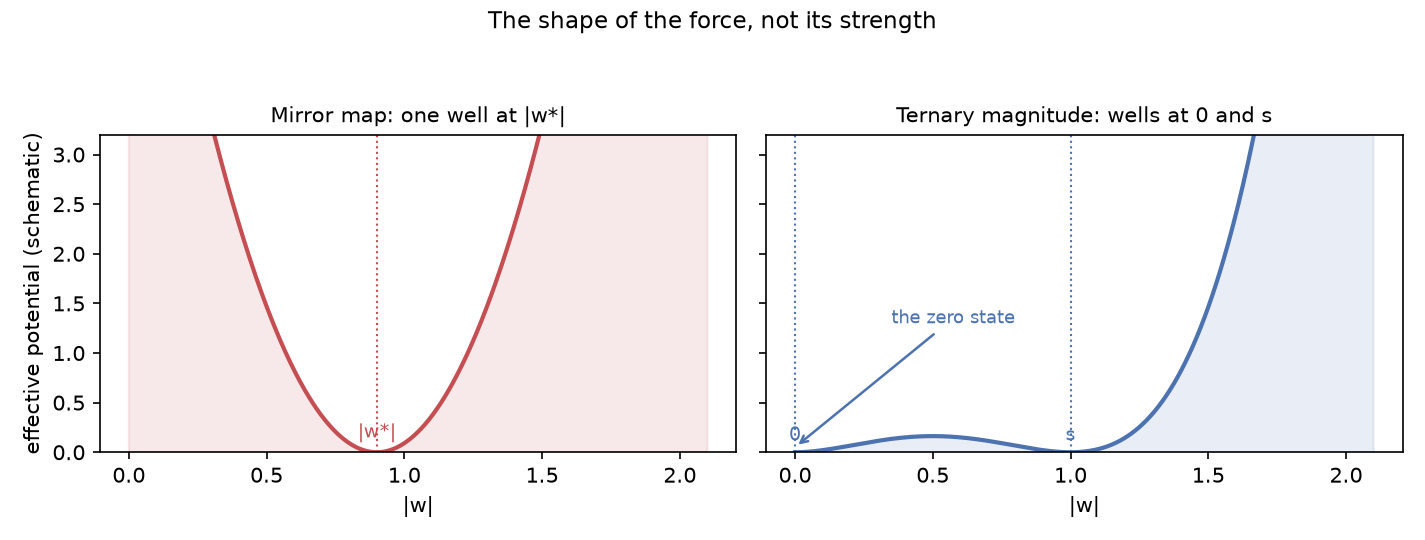
\includegraphics[width=0.85\linewidth]{figures/rmd-wells.png}
\end{center}
\caption{Schematic effective potential in magnitude. Left: the mirror map has
a single well at $|w^{\star}|$. Right: ternary needs two wells, at $0$ and
$s$; a single-well force cannot populate the zero basin.}
\label{fig:rmd-wells}
\end{figure}

\begin{figure}[t]
\begin{center}
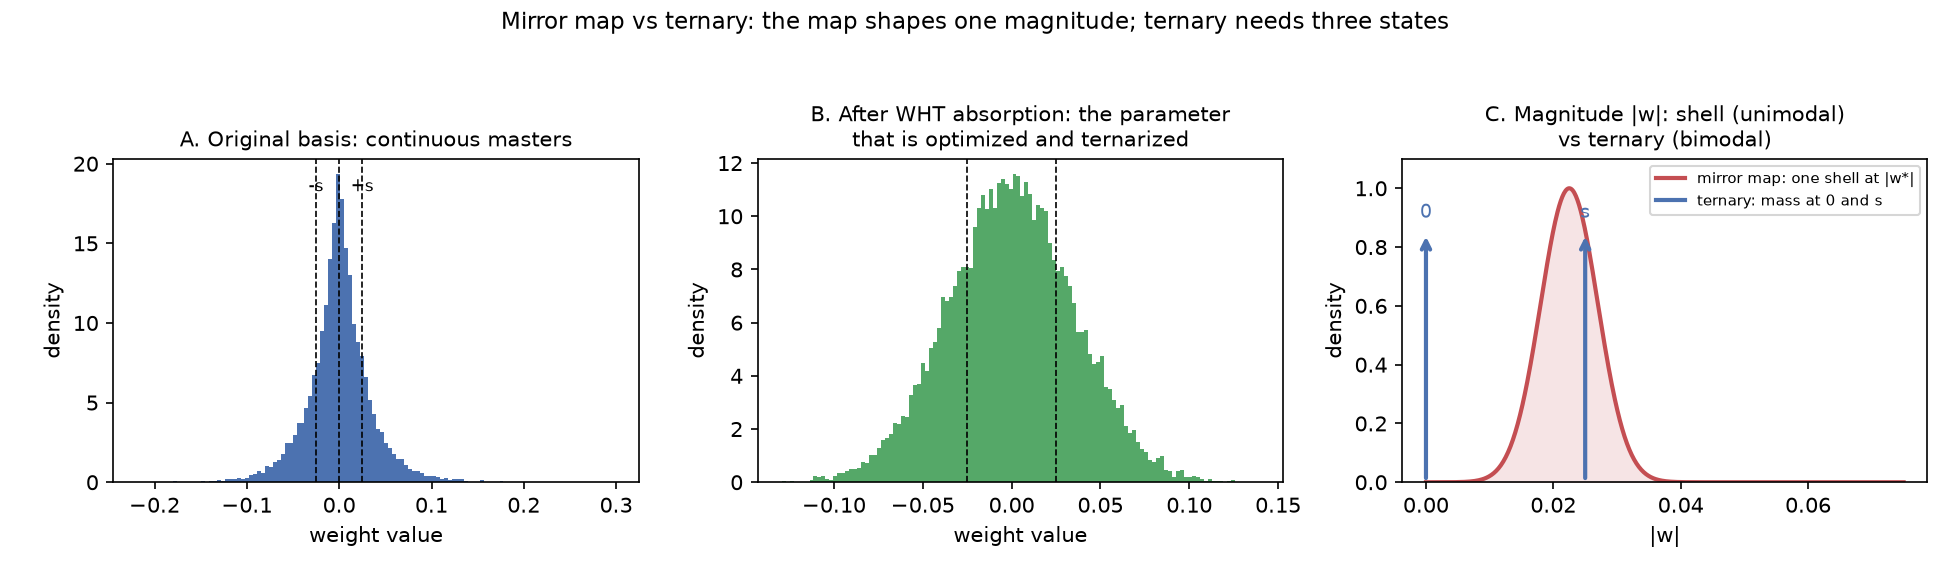
\includegraphics[width=\linewidth]{figures/rmd-shell-vs-ternary.png}
\end{center}
\caption{(A)~Continuous masters in the original basis with the ternary grid.
(B)~After the rotation is absorbed: the parameter that is optimized and
ternarized. (C)~The magnitude each method shapes; the mirror map forms one
shell, ternary needs mass at $0$ and $s$.}
\label{fig:rmd-shell}
\end{figure}

\paragraph{What the evidence supports.}
Putting the pieces together---the basis and format are public and exactly
recoverable; the residual is trained weight movement, not error compensation;
the zero band is the quantizer's band; the quality gap is total when the codes
are replaced; the mirror map fails in the loop---the best-supported account of
the release is the conventional one: \emph{rotation inside the training loop,
a ternary quantizer with a straight-through estimator, distillation from the
full-precision teacher, and a managed learning-rate schedule}. Mirror descent
belongs to the intellectual lineage of the mechanism, in particular the binary
case, but our experiments do not support it as the algorithm this model runs.

\subsection{The 1.7B pilot, and a holdout leak that retracts our own number}
\label{sec:pilot}

To price the remaining route we ran the conventional recipe on a
Qwen3-1.7B canary with the student and teacher on one card, distillation
temperature $2$, and a fixed evaluation set. The metric is the student-to-teacher
perplexity ratio (lower is better); retention is its reciprocal.

We have to open this subsection with a retraction. The first run of this pilot
reported $1.103\times$ ($90.6\%$ retention). A later audit found that the
harness sampled evaluation windows from the training pool---every evaluation
window had been seen roughly seventeen times during training---so the number
was a training-set measurement. A first correction ($1.219\times$, $82.0\%$)
turned out to be contaminated too: the holdout exclusion and the evaluation
call disagreed on sequence length, so the ``held-out'' evaluation still read
training data. Both numbers are retracted. On a clean multi-region holdout
(eight disjoint regions, $32$k tokens), the plain straight-through control sits
at $2.09\times$ mean ($\sim$48\% retention, range $1.55$--$2.71\times$). The
gap was larger than first reported, and the localization of
\S\ref{sec:mechanism} is what survives: the missing quality is training, not
quantization.

Under the clean holdout, the ablations behave as expected. Rotation inside the
loop is the single largest lever ($2.09\times \rightarrow 1.37\times$ at $5000$
steps); training longer improves it ($1.2152\times$, $82.3\%$, at $10{,}000$
steps); adding a managed decay schedule reaches $1.1052$--$1.1532\times$
($86.7$--$90.5\%$) depending on seed, though these are validation-selected
points. Corpus choice matters enormously: on WikiText~\citep{wikitext}, with an
in-distribution teacher, the same recipe at iso-convergence lands at
$1.5731\times$ ($63.6\%$) for 1.7B and $1.9263\times$ ($51.9\%$) for 0.6B,
rising with scale but far above the pre-registered bar. The 4B rung was dropped
by decision, so the scaling question is not resolved
(Figure~\ref{fig:retention}).

\begin{figure}[t]
\begin{center}
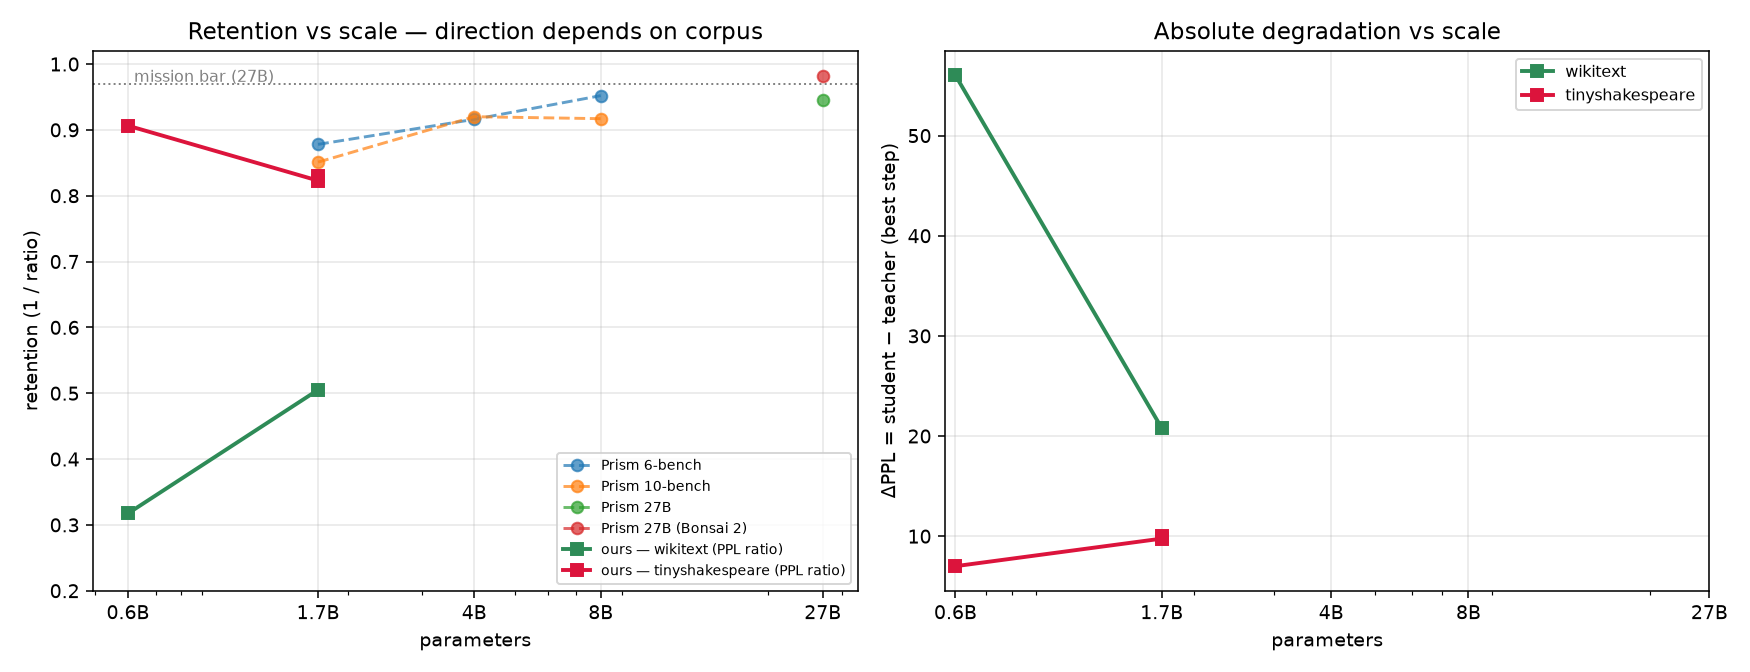
\includegraphics[width=\linewidth]{figures/retention-vs-scale.png}
\end{center}
\caption{Retention versus scale. Circles: the release's published benchmark
retention, which rises with scale. Squares: our canary's perplexity-ratio
retention on two corpora. The rulers differ (benchmark accuracy versus
perplexity ratio), so this is a same-scale sanity check, not a parity claim.}
\label{fig:retention}
\end{figure}

\paragraph{Where this leaves the gap.}
The residual that carries the quality is trained weight movement
(\S\ref{sec:mechanism}); every cheaper route has been eliminated; a local
per-layer distillation variant does not control global compounding; and the
canary, once its evaluation is clean, is further from the bar than first
stated. The remaining route to reproducing the released artifact is a full
end-to-end QAT/KD run at 27B, which we did not fund. What this study proves is
\emph{where} the gap is and what does \emph{not} close it---not that the recipe
reproduces the released numbers.

\section{Discussion}
\label{sec:discussion}

\paragraph{What a released ternary checkpoint reveals.}
Without training code, a released file still supports a surprising amount of
verification: the format, the rotation basis, the layout conventions, and the
code distribution are all measurable, and the public base makes the residual
measurable too. In this case the container turned out to be fully recoverable
from the artifact plus the base model, and the recovery later matched the
authors' published manifest exactly. Releasing format metadata is cheap and
disproportionately useful: it converts format reconstruction into verification
and lets independent parties spend their effort on the scientific question
instead.

\paragraph{Agreement is not quality.}
Ninety-two percent trit agreement sounds like a near-copy; it coexists with a
$1{,}270\times$ perplexity collapse. The mismatched codes are not noise around
a threshold, they are boundary placements that training put where the model
needs them, and they carry the model. Any pipeline that reports code agreement
as evidence of parity---ours included, before the payload-swap experiment---should treat the metric
as a container check and validate quality by a controlled swap or a held-out
evaluation.

\paragraph{Calibration hygiene is a first-class result.}
The public PTQ baseline reproduces its published figure on its calibration
passage and collapses by three to four orders of magnitude off it. This is not
a criticism of the method family but of the evaluation protocol: with
calibration-dependent methods, the calibration and evaluation sets must be
disjoint, and the disjointness must be stated. Our own protocol failures
(\S\ref{sec:pilot}) are the same disease in a different organ---an evaluation
set that was not actually held out---and they were caught only by an explicit
audit. We report the retraction because a forensic study's credibility rests on
its own error handling.

\paragraph{Fair accounting for ``about two bits per weight''.}
Effective bits per weight must count every parameter, including embeddings and
norms kept at higher precision. Ternary-only counts overstate compression: our
own otherwise ternary 1.7B recipe sat at an effective $4.53$\,bpw because the
embedding and head were not ternarized, while the released model ternarizes its
embedding, so a like-for-like comparison requires the effective number on both
sides. This matters for any claim that a PTQ method at ``2-bit'' matches a
trained ternary release.

\paragraph{Negative results, recorded.}
Several routes were eliminated: error-compensated quantization in the correct
basis, stochastic calibration resonance, continuous attractor potentials,
alternating projection, local per-layer distillation, entropy-based data
selection, and the mirror map. Each is recorded with its evidence and the cost
to revisit (Appendix~\ref{app:failures}). Two of them are informative in their
own right: the direction of the GPTQ results (compensation moves codes away)
and the mirror-map shape argument (a single-well force cannot populate a
two-well target) are general observations about ternary training, not just
statements about this model.

\paragraph{Open questions.}
Three remain. First, a full 27B end-to-end QAT/KD run, priced but not funded,
is the only route to a reproduction of the released numbers. Second, a
same-ruler comparison of trained ternary versus PTQ at matched effective bit
width, on the same base and corpus, is still missing from the public record.
Third, the extension of the forensics to mixture-of-experts models---routing
drift under ternarization and where to place corrections---is started in the
artifact but out of scope here; it is the natural next specimen, because
routing adds a failure mode that dense models do not have.

\section{Limitations and threats to validity}
\label{sec:limitations}

\paragraph{What the evidence covers.}
This is a historical forensic write-up assembled from a research programme that
has ended: the public artifact contains the scripts and reports, but not every
referenced large artifact or private-history record, so some provenance
identifiers are not reproducible from the public checkout. The numbers in the
public reports are the authoritative record for every claim here. Nothing in
this paper claims packed \texttt{PQ2\_0} parity for our own pipeline, a
completed 27B QAT run, or an unbiased final test-set claim.

\paragraph{Protocol size.}
Quality numbers use one corpus ($\sim$1.1\,MB of Shakespeare), an $8\times512$
context, one binary, and single runs per arm. Perplexity of a badly broken
model is noisy ($\pm 1231$ on $23{,}606$), and the corrected 1.7B numbers are
validation-selected points rather than pre-registered final results. The
directions and effect sizes we rely on are far outside that noise, and the
smoke arm is monotone in swap size, but absolute values should be read as
controlled comparisons rather than benchmark-grade estimates. No KLD or
downstream task evaluation is reported.

\paragraph{Coverage of the agreement analysis.}
Agreement was measured on $26$ tensors sampled from layers $0$, $3$, $62$, and
$63$ of the 27B, and the Hessian experiments use a four-layer prefix; both
choices trade coverage for feasibility, since the full model does not fit
locally. The direction of the results is uniform across tensors and layer
types, but a full-model sweep would strengthen the magnitudes.

\paragraph{The 1.7B canary is not the 27B.}
The pilot numbers describe a different model at a different scale and a
different metric (perplexity ratio rather than benchmark retention). Their
role is to price the remaining training route and to expose evaluation
failures, not to stand in for a 27B result. The same applies to the PTQ study,
which is instantiated at 1.7B: the calibration-collapse direction is what we
claim, not exact ratios at 27B.

\paragraph{Mechanism statements are bounded.}
The experiments prove that some weight movement occurred during training; they
do not identify the optimizer or prove that QAT/KD specifically produced the
released weights. ``Rotation-in-the-loop QAT/KD'' is the best-supported
account, not a demonstrated reproduction. The mirror-descent falsification is
specific to the tested configurations in the deployed metric and does not
falsify mirror descent as a family.

\paragraph{Post-hoc verification.}
The format recovery was performed before consulting the authors' published
manifest; however, we did not pre-register the recovery, so the confirmation is
post-hoc rather than a blind prediction. We report it as agreement, not as a
prediction.

\paragraph{Out of scope.}
Mixture-of-experts ternarization, speculative-drafting behaviour, and the
runtime engineering of the inference fork are out of scope; the drafter track
in the artifact is recorded there as a shelved negative result. Runtime
timings are descriptive only (the measured generation rate is below the target
we had set for our own artifact) and should not be read as a runtime
comparison.

\section{Broader impact}
\label{sec:impact}

Aggressive weight quantization lowers the compute and memory barriers to
running capable language models, which is a broadly positive development; it
also means that quality claims attached to low-bit releases can outrun what
users can verify. Independent forensics is one part of keeping that ecosystem
accountable: the ability to check, from public files, what a release actually
contains, how much of its quality is in its weights, and whether a baseline
survives off-calibration. Our findings are adversarial only in the scientific
sense---we redistribute no weights and rely on public artifacts---and we see no
direct negative societal impact specific to this study. The main risk we can
name is the inverse of its value: code-agreement or calibration-passage metrics
taken as quality guarantees. This paper documents two concrete ways that goes
wrong.

\section{Reproducibility and artifacts}
\label{sec:repro}

Every measurement in this paper is produced by scripts in the artifact, which
is available as \coderef{}. The artifact contains: the spec for the recovered
format with a canonical hash that is checked by the test suite
(\texttt{SPEC\_SHA256}, \code{0d2c008b4a9e\ldots}); byte-exact decoders for the
packed format; the rotation, layout, and agreement tooling; the controlled-swap
patcher; the Hessian capture and GPTQ variants; the evaluation harness wrapper;
offline tests that use synthetic tensors only (no downloads, CPU-only, CI
green); and the full failure register. Large artifacts---model weights,
calibration Hessians, evaluation outputs---are not redistributed; they are
regenerable from the public base and release with the commands in the artifact.
The evaluation protocol, hyperparameters, and the retraction timeline are
documented in Appendix~\ref{app:protocols}. We also note what is \emph{not}
reproducible: some provenance commit hashes refer to a private working history
and are provided for the record only.

\section{Conclusion}
\label{sec:conclusion}

We took apart a released ternary language model using only public files. The
format and the rotation basis are exactly recoverable from the release and the
public base; the last $8\%$ of codes are not, and they are the model: replacing
them with rotate-and-round weights of the base collapses perplexity by
$1{,}270\times$ in the same binary. Error-compensated quantization of the
public base cannot produce the released codes---every variant we tried moved
codes away, and the released codes fit real activation Hessians worse than
plain round-to-nearest---so the residual is weight movement from training, with
rotation-in-the-loop QAT/KD as the best-supported account and the mirror-map
recipe falsified in the deployed metric. On the evaluation side, a widely cited
public PTQ baseline reproduces its published $2.1\times$ only when calibration
and evaluation share a passage; off-calibration it collapses by three to four
orders of magnitude. We close the quantizer reverse-engineering track, retract
our own earlier 1.7B retention number after a holdout leak, and record every
falsified route so the next attempt starts from what was actually established:
the gap is localized, priced, and reachable only through end-to-end training at
scale.


\bibliography{refs}
\bibliographystyle{tmlr}

\appendix
\section{Failure register}
\label{app:failures}

The register is append-only; each entry records the claim, the method, the
outcome, and the cost to re-assess. Table~\ref{tab:register} summarizes the
load-bearing entries; the full register, including operational incidents
(\code{U1}--\code{U3}), is in the artifact.

\begin{table}[t]
\caption{Failure register (condensed). ``Status'' reflects the state at the
time of writing.}
\label{tab:register}
\begin{center}
\begin{tabular}{p{0.05\linewidth}p{0.62\linewidth}p{0.25\linewidth}}
\toprule
id & one-line outcome & status \\
\midrule
F1 & Public PTQ collapses off-calibration; the published $2.1\times$ is a calibration-passage artifact; the public stack runs $1.2\times10^{3}$--$3.5\times10^{4}\times$ held-out. & falsified, closed \\
F2 & GPTQ/Hessian variants move codes away from the released ones (RTN $0.9145$ vs $0.8086$--$0.8497$); quantizer reverse-engineering closed. & falsified, closed \\
F3 & Stochastic calibration resonance: $4.3\%$ of codes move, agreement changes $+0.003$\,pp. & falsified, closed \\
F4 & Rotate $+$ absmean RTN of the public base: $23{,}606$ vs $18.5851$ PPL ($1{,}270\times$). & falsified, closed \\
F5 & The last $\sim$$8\%$ localized to end-to-end QAT; the 27B proof-run priced and deliberately not funded. & deferred by decision \\
F6 & Student-stream block-wise distillation: $1.25$M PPL, worse than RTN. & dead end \\
F7 & Teacher-forced block-wise distillation: $1.06$M PPL; per-layer distillation compounds globally. & dead end \\
F8 & Entropy/excess-loss data selection lost to random ($172.3$ vs $115.9$ PPL). & falsified (pilot) \\
F11 & The 1.7B pilot's $1.103\times$ was measured on training windows; clean multi-region holdout is $\sim$$2.09\times$ ($\sim$48\%); both earlier corrections retracted. & retracted; open \\
\bottomrule
\end{tabular}
\end{center}
\end{table}

\section{Protocols and hyperparameters}
\label{app:protocols}

\paragraph{Decode and agreement.}
Released payloads are decoded with the byte-exact \texttt{PQ2\_0} decoder
(34\,B per 128 weights; FP16 group scale; 16 trits per 32-bit word). Agreement
is Equation~\ref{eq:agreement}, computed after mapping each public-base tensor
to the release's layout and applying the recovered rotation with the explicit
sign vectors read from the file metadata. Reported values are per-tensor means
over the sampled tensors.

\paragraph{Controlled swap.}
All $402$ mapped payloads are rewritten in place; the file's metadata,
tokenizer, tensor table, offsets, and non-ternary tensors are untouched.
Pack/unpack round-trips are byte-exact; post-patch SHA-256 verification covers
all $402$ tensors. Evaluation uses the release's fork perplexity binary at
$8\times512$ context on the fixed corpus, one process at a time, with the
device pinned.

\paragraph{Hessians and GPTQ variants.}
Embedding plus layers $0$--$3$ are loaded alone ($55$ tensors), real corpus
windows are run through them, and float32 Hessians are captured on the original
norm outputs. Each weight is layout-adjusted and rotated with the explicit
signs; GPTQ is run in that basis with damping
$\{0.01, 0.1, 0.3\}$, act-order on/off, rotation-aware ($R^{\top} H R$) versus
raw Hessians, and a group-scale search in diagonal-H and block-H forms.

\paragraph{Stochastic calibration.}
GPTQ with group size $128$ and damping $0.1$ on the 1.7B canary, with clean
versus $5\%$ random-token-noise calibration Hessians, compared against the
released 1.7B ternary codes (byte-exact decode).

\paragraph{Canary pilot and holdout.}
Qwen3-1.7B student and teacher, distillation temperature $2$, $512$-token
windows. The clean holdout is eight disjoint regions of $32$k tokens with
$8\times512$ evaluation windows per region; training windows are sampled
outside the holdout, and the evaluation call uses the same sequence length as
the holdout definition (the mismatch between the two is what contaminated the
retracted corrections). Reported pilot numbers are the best checkpoints on the
holdout, i.e.\ validation-selected, not final-test numbers.

\paragraph{Retraction timeline.}
(1) Reported $1.103\times$/$90.6\%$: training-window evaluation; retracted.
(2) Corrected $1.219\times$/$82.0\%$: holdout/evaluation sequence-length
mismatch; retracted. (3) Clean holdout: plain STE control $2.09\times$ mean;
recipe ablations as reported in \S\ref{sec:pilot}. The register entry
\code{F11} is kept open for a re-baseline rather than closed.


\end{document}
